We derive upper limits on the SM gluon-fusion Higgs boson production cross section 
times the $\hww\to 2\ell2\nu$ branching ratio in the $115 < m_H < 600 \GeVcc$ mass range. 
The results are presented in terms of the ratio of the limits to the rate predicted 
by the SM as a function of the Higgs boson mass corresponding to an integrated 
luminosity of $\intlumi$. Only expected limits are shown for the time being.

The limits are derived with a statistical method based on Bayesian
inference~\cite{bayesian}, using a likelihood function from the
expected number of observed events modeled as a Poisson random
variable whose mean value is the sum of the contributions from signal
and background processes. We account for systematic
uncertainties in a form of nuisance parameters with a log-normal
pdf. Results are reported with a flat signal {\it prior}. To perform
the computation of the limits, the software package LandS~\cite{lands}
is used.

The estimation of the backgrounds follows the strategies described in 
Section~\ref{sec:backgrounds}. Table~\ref{tab:routin_data} 
shows the results for the $\dyll$ estimation in the different jet bins. 
The fake-induced background estimation at the $\WW$ level is reported in 
Table~\ref{tab:fake_est}, while Table~\ref{tab:ttbar_est} shows the 
results for the top background estimation. 
As a summary, the expected and observed 
number of signal and background events after applying the $\WW$ selection 
requirements for each jet bin are reported in 
Table~\ref{tab:wwselection_all} and the $\mt$ distribution after the $\WW$ preselection 
is shown in Figure.~\ref{fig:ww_mt}. 



%%%%%%%%%%%%%%%%%%%%%%%%%%%%%%
\begin{table}
\begin{center}
\begin{tabular}{c c c c}
\hline
\vspace{-3mm} && \\
analysis   & $N_{out} (data/MC) 0-jet$ & $N_{out} (data/MC) 1-jet$ & $N_{out} (data/MC) 2-jet$  \\
\vspace{-3mm} && \\
\hline
$\WW$&     3.27 $\pm$ 2.89 &     4.17 $\pm$ 2.46 &     6.49 $\pm$ 1.94\\\hline
 115 &    6.92 $\pm$ 5.32  &    2.09 $\pm$ 3.52  &    5.44 $\pm$ 4.77 \\
 120 &     7.44 $\pm$ 5.88 &    3.18 $\pm$ 5.32  &    2.75 $\pm$ 2.67 \\
 130 &     2.01 $\pm$ 4.87 &    2.78 $\pm$ 6.97  &    2.40 $\pm$ 2.70 \\
 140 &     1.41 $\pm$ 4.90 &     2.71 $\pm$ 6.74 &    2.86 $\pm$ 3.13 \\
 150 &     3.95 $\pm$ 8.81 &    3.92 $\pm$ 6.82  &   8.58 $\pm$ 14.30 \\
 160 &    0.67 $\pm$ 2.63  &    3.14 $\pm$ 4.75  &   7.77 $\pm$ 11.54 \\
 170 &    0.41 $\pm$ 6.94  &    4.00 $\pm$ 5.94  &  11.32 $\pm$ 19.90 \\
 180 &    0.81 $\pm$ 2.68  &    1.54 $\pm$ 3.22  &    9.32 $\pm$ 13.04\\
 190 &  25.82 $\pm$ 49.70  &    4.19 $\pm$ 7.68  &     8.94 $\pm$ 6.45\\
 200 &   1.95 $\pm$ 13.42  &    4.47 $\pm$ 7.51  &     8.55 $\pm$ 5.44\\
 250 &    0.49 $\pm$ 3.97  &    3.73 $\pm$ 2.27  &     7.71 $\pm$ 2.54\\
 300 &    0.85 $\pm$ 4.77  &    3.90 $\pm$ 3.71  &     7.14 $\pm$ 1.88\\
\hline
\end{tabular}
\caption{The Drell-Yan estimation in the same flavor final state.
\label{tab:routin_data}}
\end{center}
\end{table}
%%%%%%%%%%%%%%%%%%%%%%%%%%%%%%
\begin{table}[ht!]
\begin{center}
\begin{tabular}{c c c c c c} 
\hline
jet-bin &	 $\mu\mu$ &	 $\mu e$ &	 $e\mu$ &	 $ee$ &	 total \\ 
\hline
0 &	 4.4 $\pm$ 1.5 &	 10.5 $\pm$ 1.5 &	 27.2 $\pm$ 2.6 &	  9,1 $\pm$ 0.9 &  51.2 $\pm$ 3.5 \\
1 &	 4.5 $\pm$ 1.5 &	  7.8 $\pm$ 1.2 &	 21.5 $\pm$ 2.3 &	  3.5 $\pm$ 0.6 &  37.3 $\pm$ 3.1 \\
2 &	 1.6 $\pm$ 0.9 &	  3.1 $\pm$ 0.9 &	  8.6 $\pm$ 1.5 &	  1.4 $\pm$ 0.4 &  14.7 $\pm$ 2.1 \\
\hline
\end{tabular}
\caption{Predictions of the fake-induced background contribution 
in the data-driven estimation after the $\WW$ preselection. 
The analyzed data correspond to $\intlumi$, where the reported uncertainties are statistical only.}
\label{tab:fake_est}
\end{center}
\end{table}
%%%%%%%%%%%%%%%%%%%%%%%%%%%%%%
\begin{table}[ht!]
\begin{center}
\begin{tabular}{l c c c}
\hline
                                              &   0-jet          & 1-jet            & 2-jet\\
\hline
Monte Carlo to data scale factor  	      &  0.98 $\pm$ 0.26 & 1.01 $\pm$ 0.08 & 1.19 $\pm$ 0.50 \\
\hline
\end{tabular}
\caption{Monte Carlo to data scale factor for the top background contribution for $\intlumi$.}
\label{tab:ttbar_est}
\end{center}
\end{table}
%%%%%%%%%%%%%%%%%%%%%%%%%%%%%%

\begin{table}[ht!]
  \begin{center}
 {\small
  \begin{tabular} {|c|c|c|c|c|c|}
\hline
          &   data & all bkg. & $qq \to \WW$ & $gg \to \WW$ &  $\ttbar+tW$ \\
  \hline
  \hline
 0-jet &  617 & 571.2 $\pm$  5.5  & 415.4 $\pm$ 2.3 & 25.9 $\pm$   0.3 &  49.1 $\pm$ 0.9 \\
 1-jet &  404 & 384.6 $\pm$  4.8  & 158.7 $\pm$ 1.4 &  9.1 $\pm$   0.2 & 138.8 $\pm$ 1.3 \\
 2-jet &  257 & 272.5 $\pm$ 11.9  &  51.4 $\pm$ 0.8 &  1.7 $\pm$   0.1 & 143.7 $\pm$ 1.2 \\
 \hline
 \hline
  \end{tabular}
  \begin{tabular} {|c|c|c|c|c|}
\hline
       & $WZ$/$ZZ$ not included in the $\dyll$ & $\dyll+WZ+ZZ$ & $\Wjets$& $W+\gamma$ \\
  \hline
  \hline
 0-jet &   8.9 $\pm$	0.1 & 16.8 $\pm$   3.3 &  51.2 $\pm$ 3.5  & 2.8 $\pm$	1.0 \\
 1-jet &   9.9 $\pm$	0.2 & 17.8 $\pm$   2.8 &  37.3 $\pm$ 3.1  & 3.7 $\pm$	1.5 \\
 2-jet &   4.2 $\pm$	0.1 & 46.6 $\pm$  11.7 &  14.7 $\pm$ 2.1  & 2.7 $\pm$	1.2 \\
 \hline
 \hline
  \end{tabular}
  }
  \caption{Expected number of signal and background events from the data-driven methods for 
  an integrated luminosity of \intlumi after applying the $\WW$ selection requirements. 
  Only statistical uncertainties on the processes are reported.}
   \label{tab:wwselection_all}
  \end{center}
\end{table}

\begin{figure}[hbt]
\begin{center}
\subfigure[]{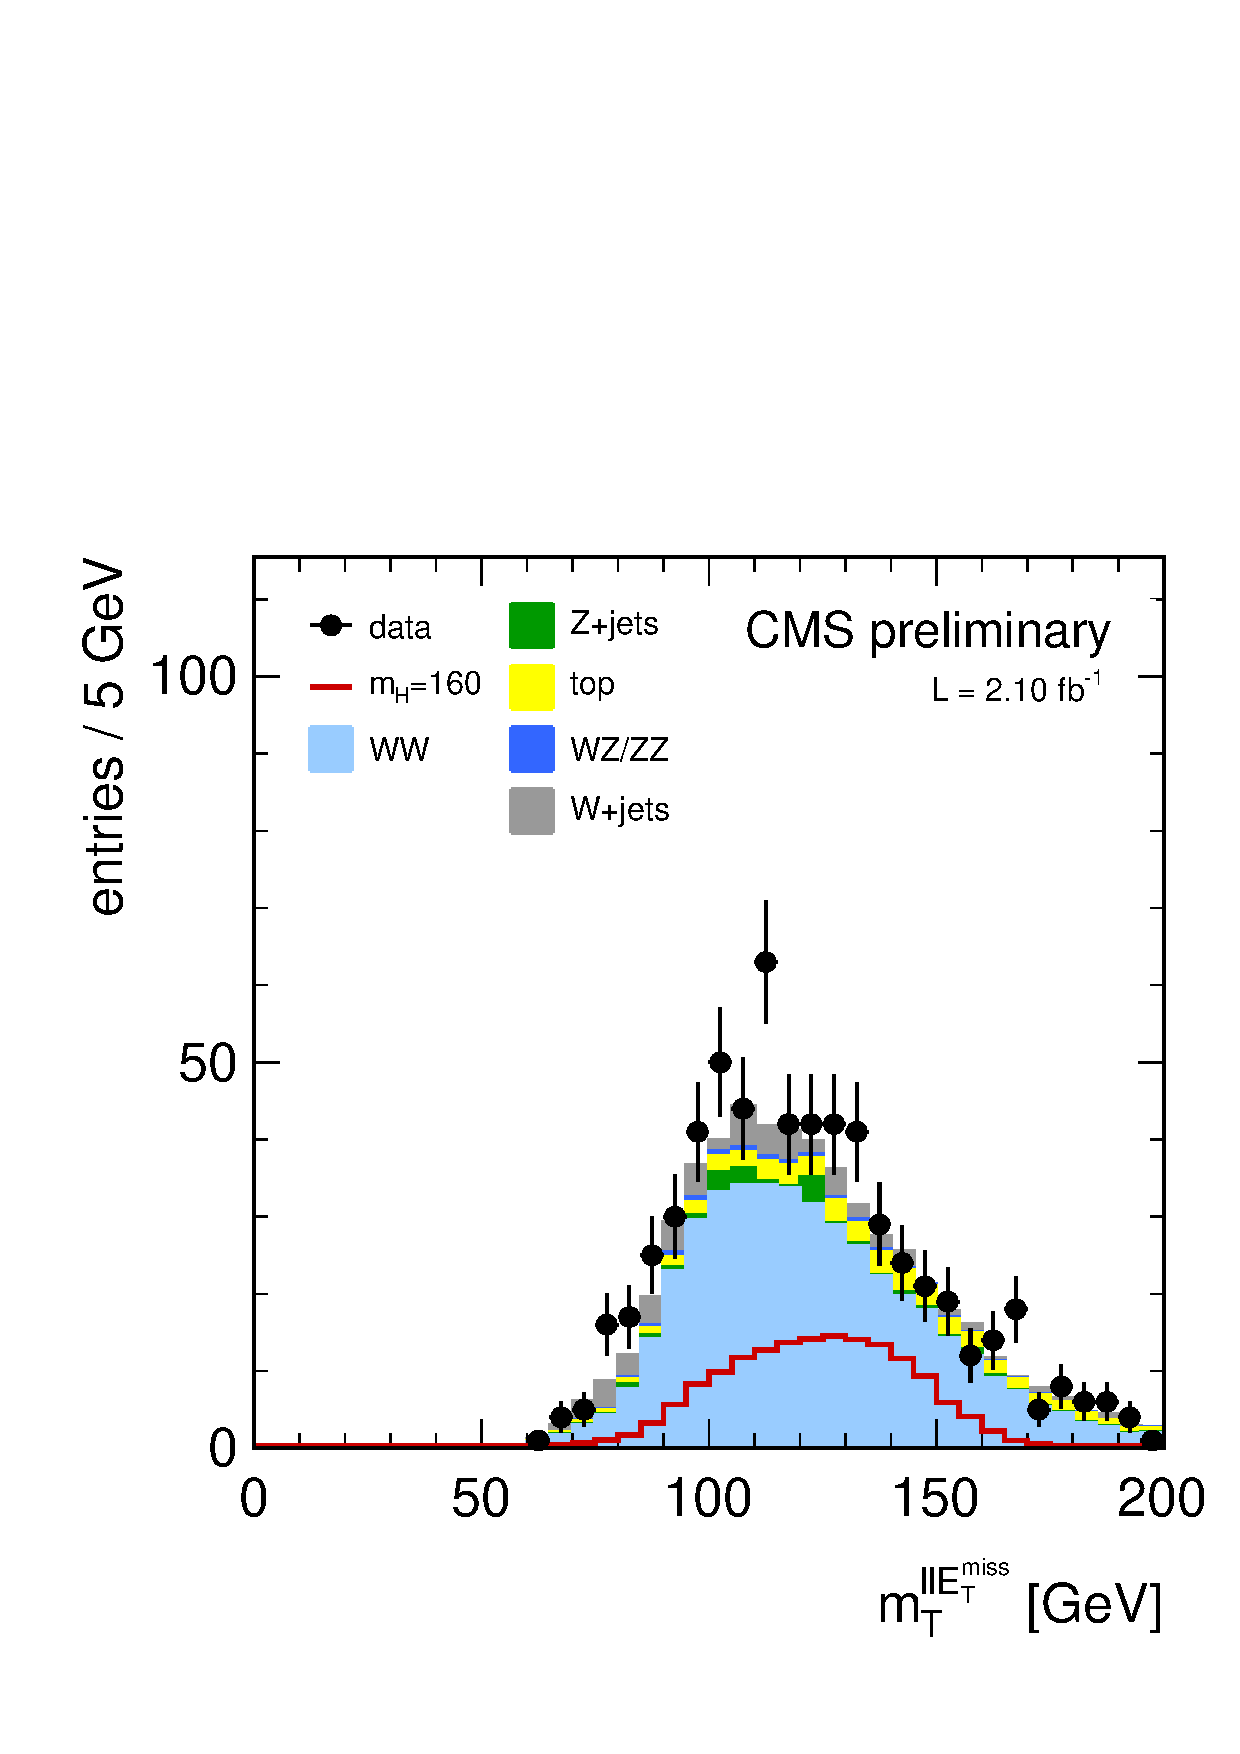
\includegraphics[width=0.49\textwidth]{figures/histo_mthiggs_ww0j_wwcuts.pdf}}
\subfigure[]{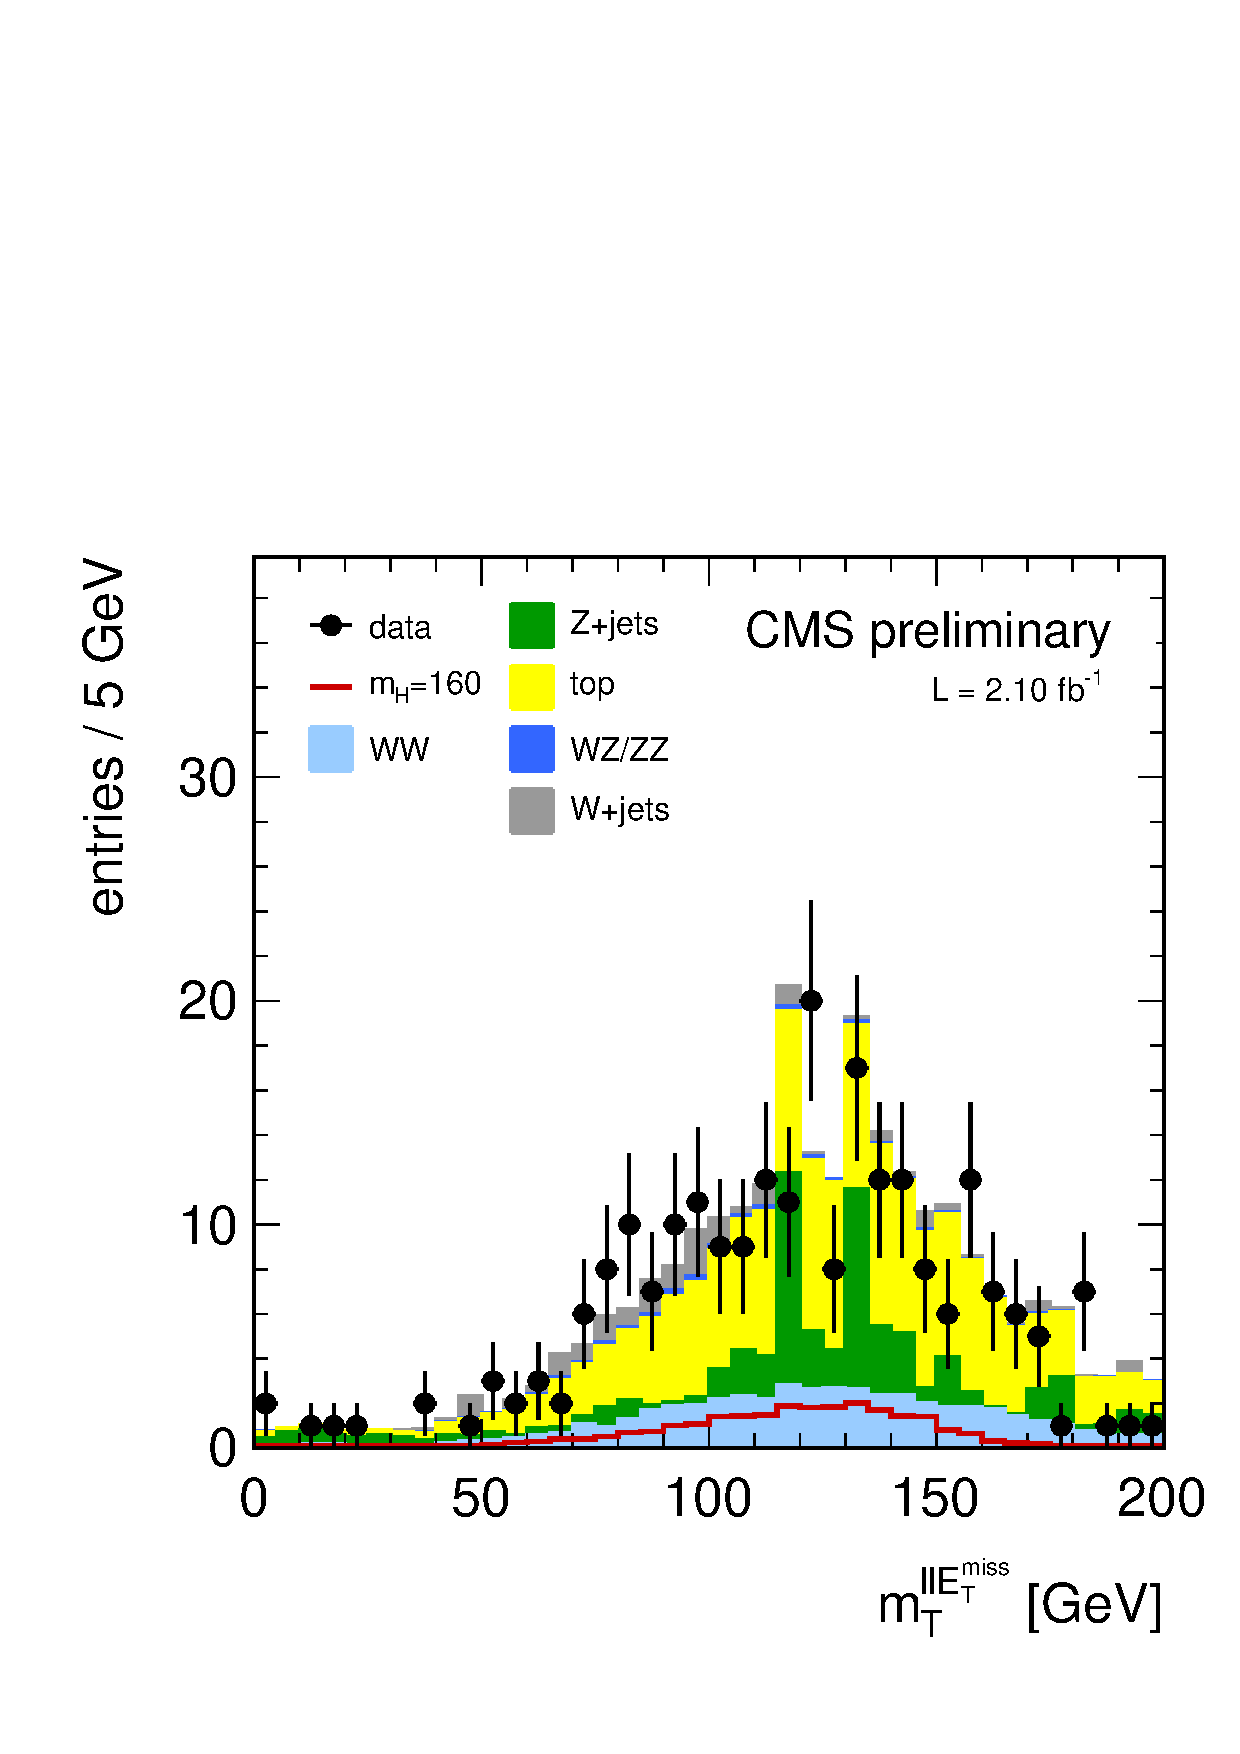
\includegraphics[width=0.49\textwidth]{figures/histo_mthiggs_ww2j_wwcuts.pdf}}
\subfigure[]{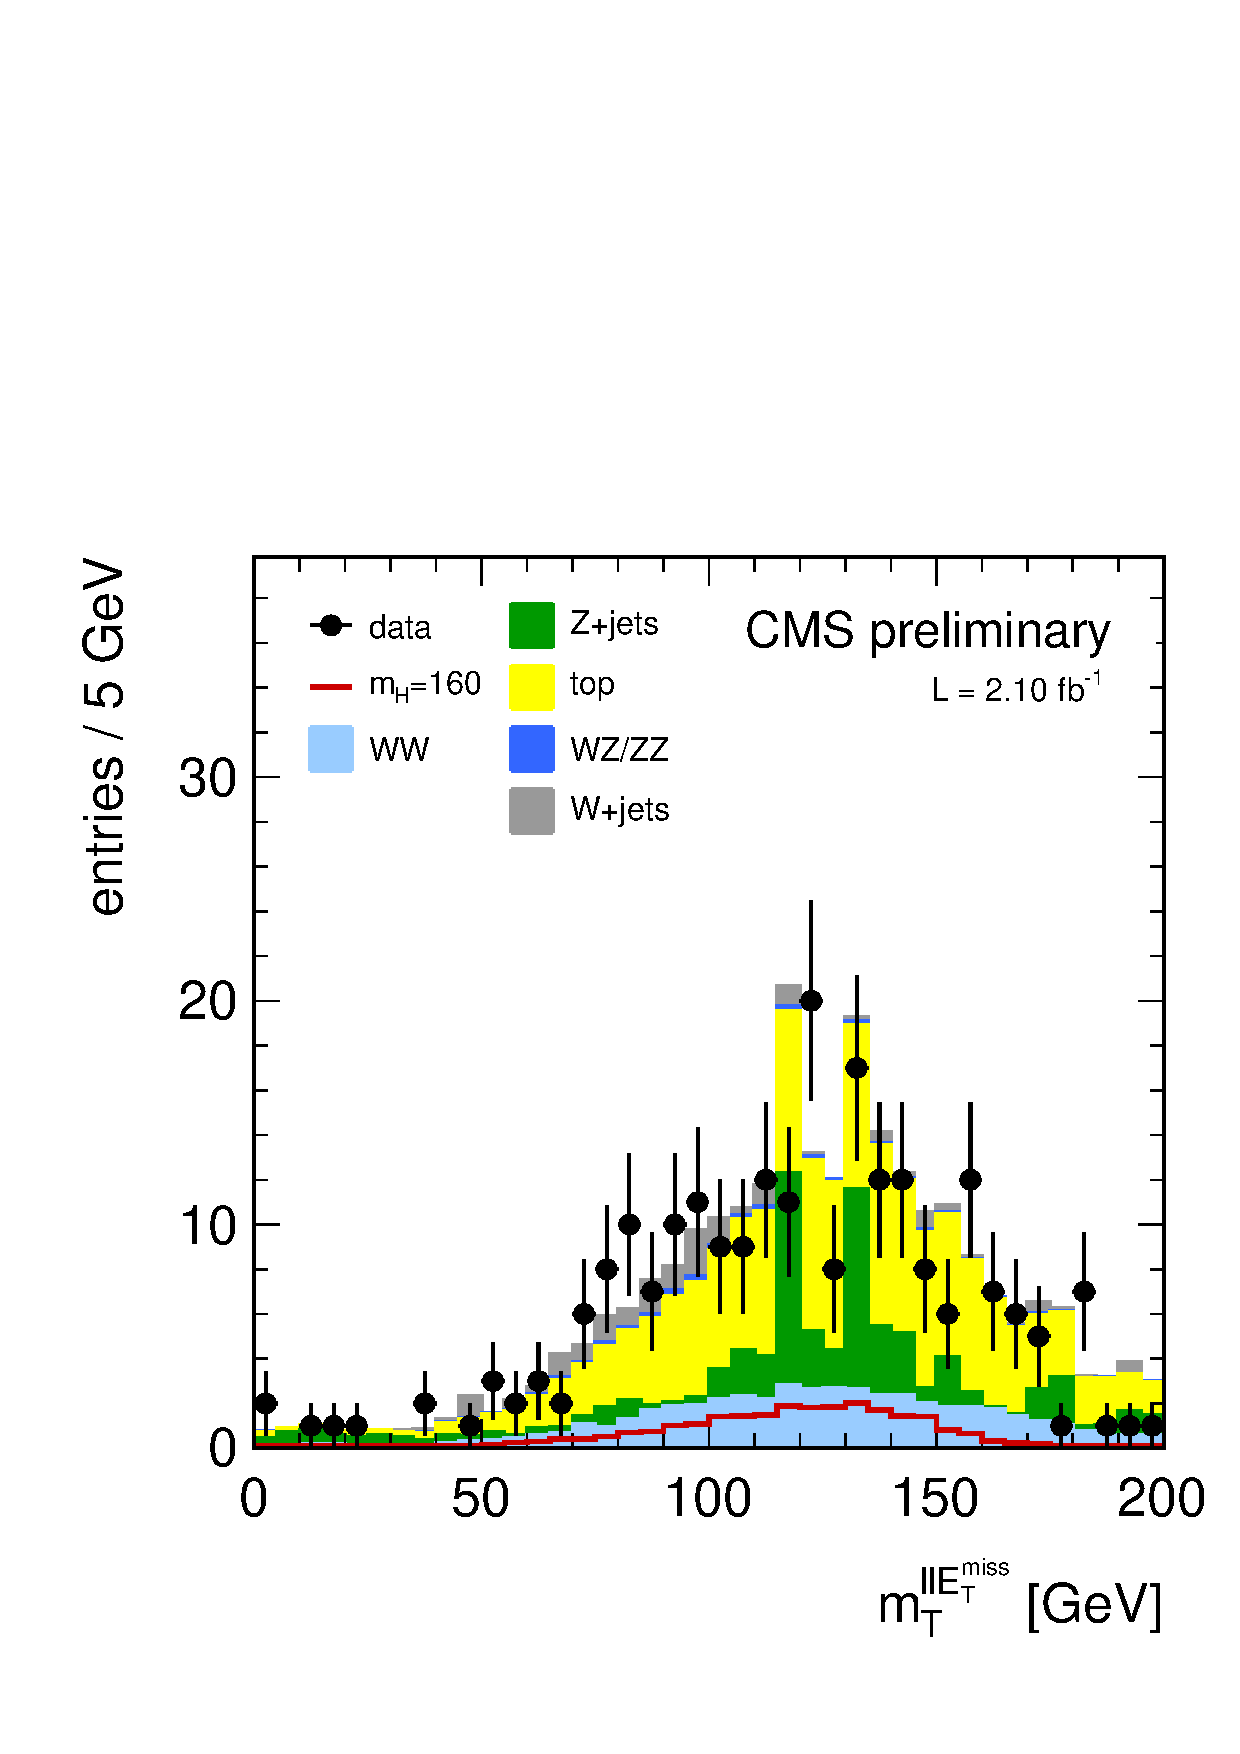
\includegraphics[width=0.49\textwidth]{figures/histo_mthiggs_ww2j_wwcuts.pdf}}
\caption{$\mt$ distribution for signal and background events after 
the $\WW$ preselection with $\intlumi$ for the three jet-bins.}
\label{fig:ww_mt}
\end{center}
\end{figure}

The expected upper limits at 95\% C.L. for the cut based and multivariate 
analyses are shown in Tables~\ref{tab:cutbase_uls} and~\ref{tab:mvabase_uls}, 
respectively.

\begin{table}[ht!]
  \begin{center}
  \begin{tabular} {|c|c|c|c|}
  \hline
cuts    & Median     &   68\%      &   95\%	 \\
        & expected   &   C.L. band &   C.L. band \\
  \hline
115 &  3.9 & [2.7, 5.6] & [1.9, 8.0] \\
120 &  2.3 & [1.5, 3.3] & [1.1, 4.8] \\
130 &  1.0 & [0.7, 1.5] & [0.4, 2.4] \\
140 &  0.6 & [0.4, 1.0] & [0.3, 1.6] \\
150 &  0.5 & [0.3, 0.7] & [0.2, 1.0] \\
160 &  0.3 & [0.2, 0.4] & [0.1, 0.6] \\
170 &  0.3 & [0.2, 0.5] & [0.1, 0.7] \\
180 &  0.4 & [0.3, 0.6] & [0.2, 0.9] \\
190 &  0.6 & [0.4, 0.9] & [0.3, 1.3] \\
200 &  0.7 & [0.5, 1.1] & [0.4, 1.5] \\
250 &  1.5 & [1.0, 2.1] & [0.8, 2.9] \\
300 &  1.7 & [1.2, 2.5] & [0.9, 3.5] \\
350 &  1.6 & [1.1, 2.3] & [0.8, 3.3] \\
400 &  1.8 & [1.3, 2.6] & [0.9, 3.6] \\
450 &  2.3 & [1.6, 3.4] & [1.2, 4.7] \\
500 &  3.4 & [2.4, 5.0] & [1.8, 7.0] \\
550 &  4.8 & [3.4, 7.0] & [2.5, 10.1] \\
600 &  7.1 & [5.0, 10.3] & [3.6, 14.9] \\
  \hline
  \end{tabular}
\caption{Expected upper limits at 95\% C.L. for the cut based analysis for an 
integrated luminosity of $\intlumi$.}
\label{tab:cutbase_uls}
  \end{center}
\end{table}

\begin{table}[ht!]
  \begin{center}
  \begin{tabular} {|c|c|c|c|}
  \hline
cuts    & Median     &   68\%      &   95\%	 \\
        & expected   &   C.L. band &   C.L. band \\
  \hline
115 &  2.9 & [1.8, 4.6] & [1.1, 7.3] \\
120 &  1.7 & [1.0, 2.8] & [0.6, 4.3] \\
130 &  0.8 & [0.5, 1.4] & [0.3, 2.1] \\
140 &  0.5 & [0.3, 0.8] & [0.2, 1.3] \\
150 &  0.3 & [0.2, 0.6] & [0.1, 0.9] \\
160 &  0.2 & [0.1, 0.3] & [0.1, 0.5] \\
170 &  0.2 & [0.1, 0.4] & [0.1, 0.6] \\
180 &  0.3 & [0.2, 0.5] & [0.1, 0.8] \\
190 &  0.5 & [0.3, 0.8] & [0.2, 1.2] \\
200 &  0.6 & [0.3, 0.9] & [0.2, 1.3] \\
250 &  1.4 & [0.9, 2.2] & [0.6, 3.2] \\
300 &  1.2 & [0.8, 2.0] & [0.5, 3.0] \\
350 &  1.2 & [0.7, 1.8] & [0.5, 2.8] \\
400 &  1.3 & [0.8, 2.0] & [0.6, 2.9] \\
450 &  1.8 & [1.2, 2.7] & [0.8, 4.1] \\
500 &  2.5 & [1.7, 3.9] & [1.2, 5.9] \\
550 &  3.7 & [2.4, 5.6] & [1.6, 8.7] \\
600 &  5.2 & [3.3, 8.1] & [2.1, 12.7] \\
  \hline
  \end{tabular}
\caption{Expected upper limits at 95\% C.L. for the multivariate analysis for an 
integrated luminosity of $\intlumi$.}
\label{tab:mvabase_uls}
  \end{center}
\end{table}
